\newcounter{qasection}
\newcounter{qaitem}
\newcommand{\qa}[2]{\stepcounter{qaitem}{\bf Q \theqasection.\theqaitem: #1}

  \medskip

  #2

  \bigskip}

\section{Questions and answers}
\label{qa}
\stepcounter{qasection}

This section answers some general questions on dvdisaster. There is also
a sub section about \tlnk{qa-technical}{technical questions}, and one
discussing \tlnk{qa-error}{error messages}.

\bigskip

\qa{How is ``dvdisaster'' pronounced?}
   {Since the word stems from the english language, simply spell ``dv'' before saying ``disaster''. Perhaps ``dee-vee-disaster'' is a suitable phonetic circumscription. }



\qa{What are quality scans and why don't you support more?}
   {\label{qa-quality-scans}Optical media have a built-in error correction which is similar
     to the method used in dvdisaster. Some drives can report the number
     of errors corrected while reading a medium. This provides a rough
     estimate of the writing and media qualities.

     \smallskip
     
     Since dvdisaster is free software, it can only include code and
     information which can be redistributed freely. This is currently
     true for C2 \tlnk{howto-scan}{scanning} of CD media, which
     is officially standardized
     and has free documentation available.

     \smallskip
     
     On the other hand, DVD quality scans (``PI/PO scans'') and BD disc
     scans are not standardized. Those drive vendors who support it are
     using proprietary programming interfaces. The respective specifications
     seem not to be available for use in free software. So we must patiently
     wait until manufacturers understand that having free software available
     for a drive will sell more drives. }

\qa{Is dvdisaster compatible with future releases?}
   {Yes, dvdisaster files are intended for an archival time of many years.
     When upgrading to a newer version of dvdisaster you can continue using
     images and error correction data created from previous versions. There
     is no need to recreate them again. }

 \qa{Augmented images have the error correction data appended at the end of the medium. Isn't that a bad choice?}
    {\label{qa-ecc-distribution}No. First a bit of terminology: If we augment 80 bytes of user data with 20 bytes
      of error correction (ecc) data, we get an ``ecc block'' comprised of 100 bytes.
      Now take the following into consideration about the ecc block:

      \begin{enumerate}
        \item The position of the error correction data within the ecc block does not matter.

          The Reed-Solomon (RS) decoder does not differentiate between user data and error
          correction data. In the view of the RS decoder our ecc block is a sequence of
          100 bytes from which an arbitrary subset of 20 bytes can be recovered. It can
          recover the first 20 bytes, the last 20 bytes, or any combination from within
          as long as the remaining 80 bytes are still intact. From this it follows that
          the position of the ecc data within the ecc block does not matter; whether it
          is appended at the end of the user data or is interleaved with it has no
          influence on the error correcting capability.

        \item Properly distributing the ecc block offsets influence of bad media spots.

          Optical media have a higher probability of failing in the outer area; but for
          technical reasons this is the only place where the error correction data
          can be stored. However this effect is offset by distributing the ecc block
          content over the medium. Let's assume that our medium is filled 80\% with
          user data, leaving the remaining 20\% free for error correction data.
          Now consider the 100 byte ecc block again. We need to pick 80 bytes from
          the user data for it and require 20 additional byte positions in the error
          correction data area. Even under these constraints it is possible to evenly
          distribute the 100 bytes over the medium, from the inside to the outside,
          each having a maximum distance to its neighbors. This means that under the
          above scenario, 80\% of each ecc block comes from the first 80\% of the medium,
          and 20\% from the rest (the outer area). Together with point (1), this negates
          the influence of bad spots on the medium. Symmetry implies that for each error
          correction byte stored in the (bad) outer region there will be a user data
          byte located in the (good) inner medium region.

          \smallskip
          
          (If you do not already see the point, imagine putting the ecc data into the
          inner medium region and the user data in the outer region. Consider point (1)
          again to see that nothing changes with respect to the error correction.)
      \end{enumerate}}

 \qa{What's the difference between image based and file based data recovery?}
    {\label{qa-image-level}Optical media are comprised of 2048 byte-wide sectors. Most of those
      sectors are used to store file data, but some of them hold
      so-called ``meta data'', e.g. information on directory folders.

      In figure \ref{qa-metadata1} (below) there is a directory ``Pics'' holding
      three files ``forest.jpg'', ``rock.jpg'' and ``protect.par''\footnote{No
        offense intended against the PAR/PAR2 project. Carsten is just confident
        that file based protection does not work on optical media :-)}.
      Note how these files are mapped onto physical sectors (green/blue
      squares) on the medium, and that an additional meta data sector
      (red square) is needed for storing the ``Pics'' directory structure.

\begin{figure}[h]
\centerline{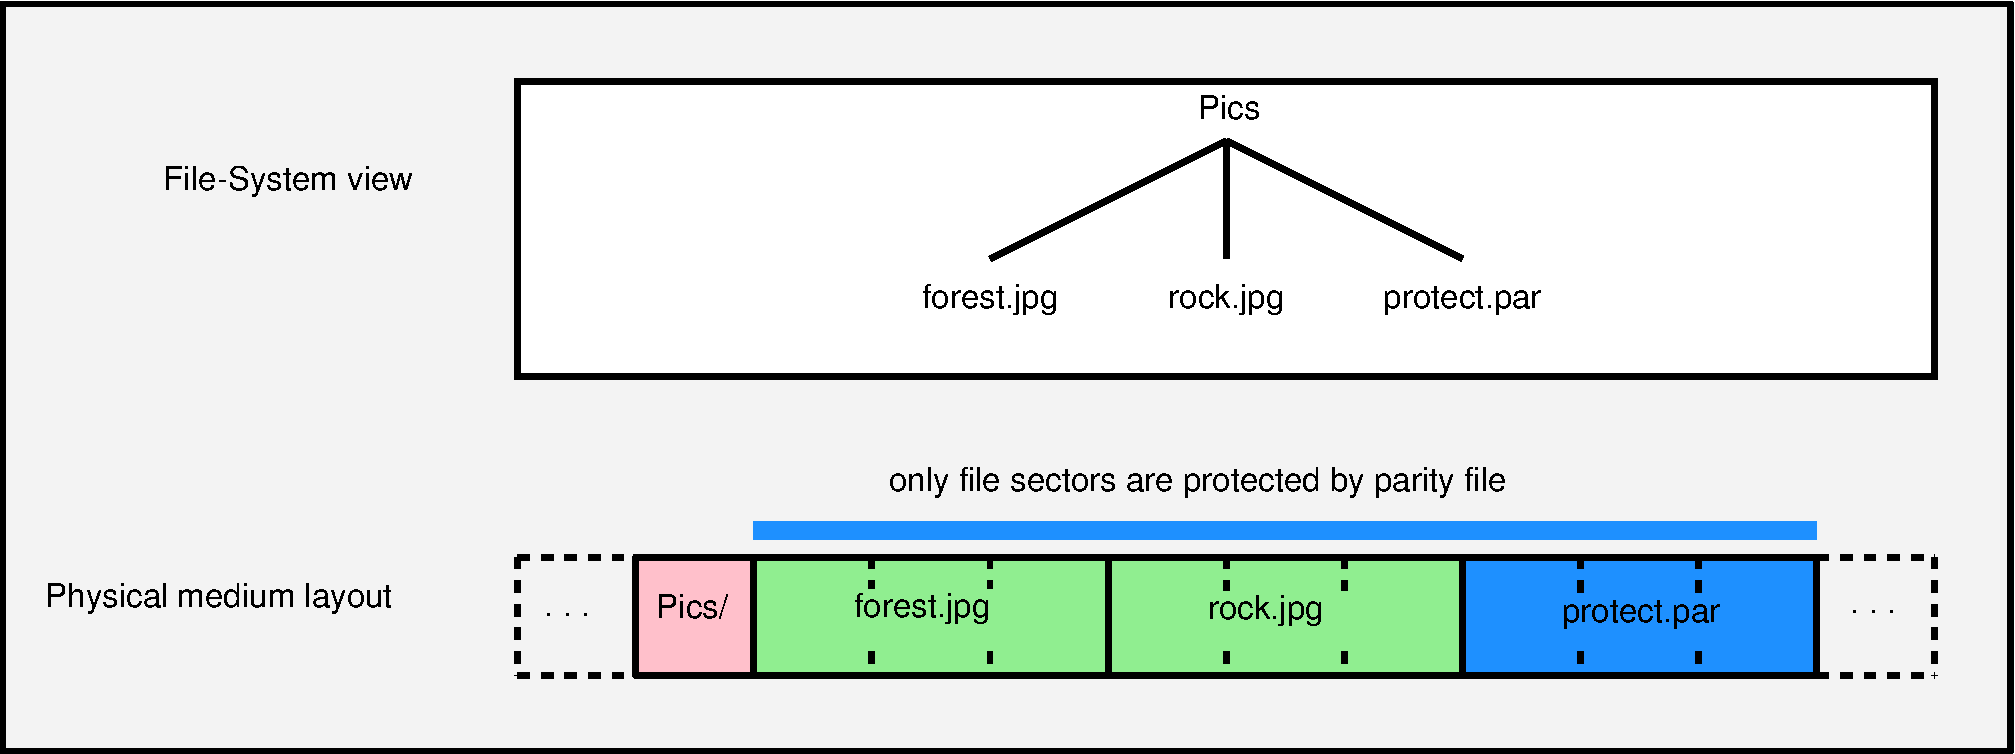
\includegraphics[width=\textwidth]{figures/metadata1.pdf}}
\caption{Relation between file system and sectors on the medium.}  
\label{qa-metadata1}
\end{figure}

\paragraph{Shortcoming of file based recovery on optical media.} Now let's assume
that we are working with file based error correction. The file ``protect.par'' holds
error correction information which can be used to recover unreadable sectors within the
files ``forest.jpg'' and ``rock.jpg''. This will only work as long as we need to
recover sectors which are part of a file. But if meta data sectors become unreadable,
the file based protection will collapse. Consider figure \ref{qa-metadata2}.
When the red directory sector becomes unreadable, not only the
directory ``Pics'' but also all files under ``Pics'' become inaccessible.
This is due to the logical structure of the ISO/UDF file system, as there is
no way to tell how the green and blue sectors relate to files anymore when
the directory is lost. So we have a complete data loss although all sectors
comprising the files are still physically readable.

\begin{figure}[h]
\centerline{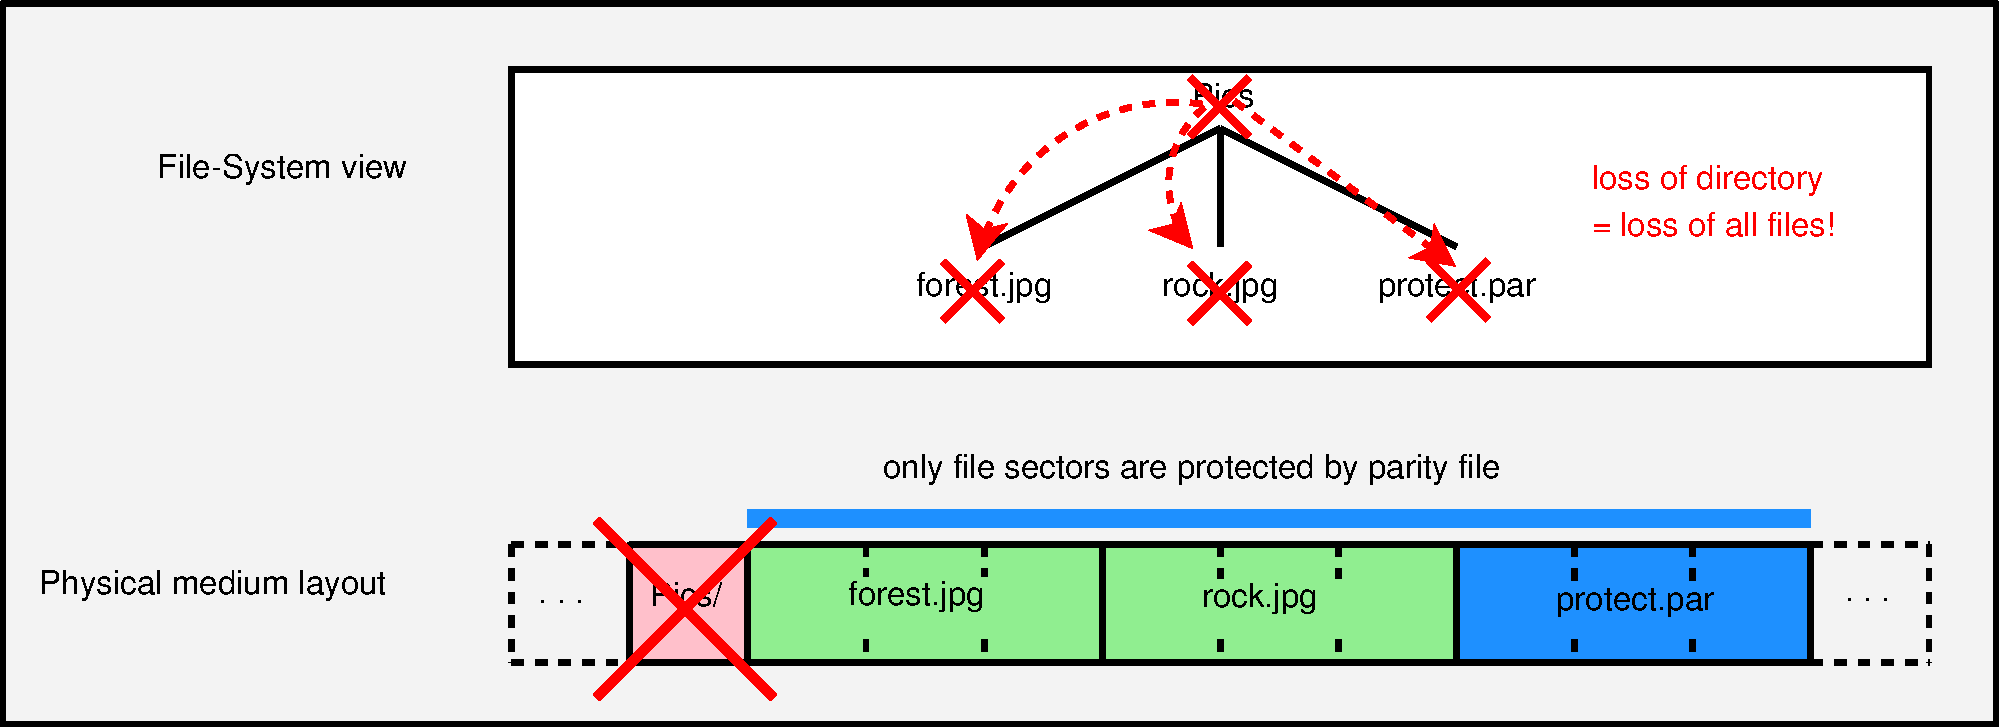
\includegraphics[width=\textwidth]{figures/metadata2.pdf}}
\caption{Losing the metadata sector produces complete data loss.}  
\label{qa-metadata2}
\end{figure}

Please note that moving ``protect.par'' to a separate medium does not rectify
the problem - the directory block is still not recoverable as it is not
protected by the error correction data in ``protect.par''.

\paragraph{Advantages of image level recovery on optical media.} dvdisaster applies
an image level approach to error recovery. The medium is read and processed as an ISO
image. The ISO image contains a sequence of all sectors found on the medium, including
those which are meta data for the file system. Since the dvdisaster error correction
data protects all sectors in the ISO image, file contents as well as meta data
sectors (e.g. directories) can be restored. See fig. \ref{qa-metadata3} for the
different range of protection. 

\begin{figure}[h]
\centerline{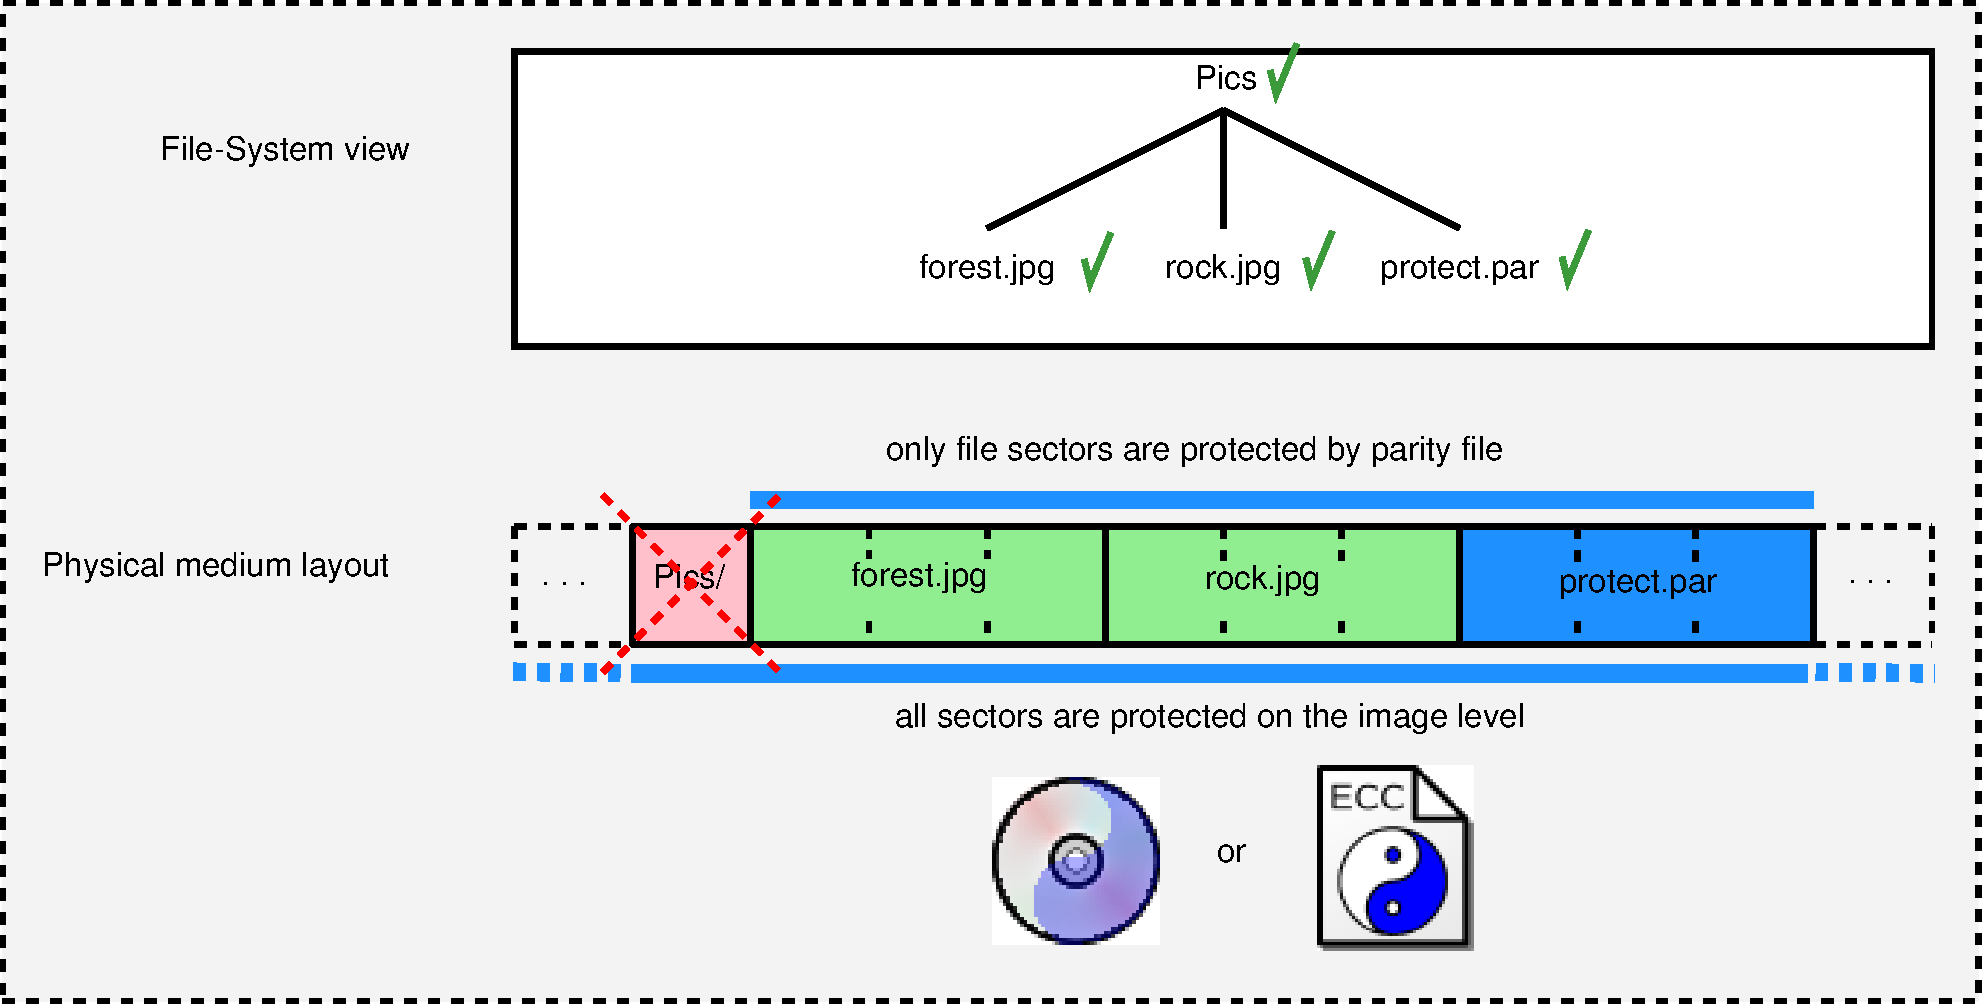
\includegraphics[width=\textwidth]{figures/metadata3.pdf}}
\caption{Image level protection}  
\label{qa-metadata3}
\end{figure}

In addition, neither reading the damaged ISO image nor applying the error
correction requires any information from the file system contained on the
medium. As long as the drive is still able to recognize the medium, dvdisaster
will be able to recover the still readable sectors from it. Therefore there are
no ``single sectors of failure'' as in the file based approach. }

\newpage
\subsection{Technical questions}
\label{qa-technical}
\stepcounter{qasection}
\setcounter{qaitem}{0}

\qa{Which on-screen translations of the program are available?\label{qa-locale}}
{The current version of dvdisaster contains screen texts in the following languages:

\medskip
  
\begin{tabular}{lll}
Czech &--& unmaintained and outdated\\
English &--& complete\\
German &--& complete\\
Italian &--& unmaintained and outdated\\
Portuguese &--& unmaintained and outdated\\
Russian &--& unmaintained and outdated\\
Swedish &--& unmaintained and outdated\\
\end{tabular}

\medskip
  
Translators for other languages are welcome!

\bigskip

dvdisaster will automatically obtain language settings from the operating system.
If the local language is not yet supported, english text will be used. A different
language can be selected using environment variables.

\medskip

Example for the bash shell and german language:

\smallskip

{\tt export LANG=de\_DE.utf8}

\medskip

Please note that we are currently not providing translations of this user manual
and the internet site. See \tlnk{qa-translate}{topic Q 2.5} for more details. 
}

\qa{Which media types are supported?}
{\label{qa-technical-media} dvdisaster supports (re-)writeable CD, DVD and BD media.
  Media containing multiple sessions or copy protection can {\em not} be used.

\bigskip
  
Usable media by type:

\medskip

{\bf CD-R, CD-RW}

\begin{itemize}
  \item only Data CD are supported.
\end{itemize}

\medskip

{\bf DVD-R, DVD+R}

\begin{itemize}
\item No further limitations are known.
\end{itemize}

\medskip

{\bf DVD-R DL, DVD+R DL (two layers)}

\begin{itemize}
\item The drive must be able to \tlnk{qa-identify}{identify (Q3.5)} the medium
  type. Typically this is only the case for drives which
  can also write two layered media.
\end{itemize}

\medskip

{\bf DVD-RW, DVD+RW}

\begin{itemize}
\item Some drives report \tlnk{qa-rw}{wrong image sizes (Q3.4)}.

  Remedy: Determine the image size from the ISO/UDF file system or the ECC data.
\end{itemize}

\medskip

{\bf DVD-RAM}

\begin{itemize}
\item Usable only when written with ISO/UDF images like DVD-R/-RW;
\item Not supported when used as removeable medium for packet writing.
\item Similar issues with \tlnk{qa-rw}{image size recognition (Q3.4)} as noted above.
\end{itemize}

\medskip

{\bf BD-R, BD-RW} \quad (one or two layers)

\begin{itemize}
\item No limitations are known.
\end{itemize}

\medskip

{\bf BDXL-R}

\begin{itemize}
\item Currently only the three-layered (100GB) version is tested and supported.
\item Note: BDXL is not backwards compatible with standard BD drives.
\end{itemize}

\medskip

{\bf Not usable types} (image can not be extracted):

\begin{itemize}
\item BD-ROM (pressed BDs), DVD-ROM (pressed DVDs), CD-Audio and CD-Video.
\end{itemize}}

\qa{Which file systems are supported?}
   {dvdisaster works exclusively on the image level which is accessed
     sector-wise. That means it does not matter with which file system
     the medium has been formatted. See also \tlnk{qa-image-level}{Q1.5}.

     \smallskip
     
     Since dvdisaster neither knows nor uses the file system structure,
     it can not repair logical errors at the file system level. It can not
     recover lost or deleted files. }

\qa{What happened to the Windows and Mac OS ports?}
   {\label{qa-discontinued-os}As you may have noticed, the project has progressed very slowly in the
     last years. The main developer is currently very short of time,
     and some co-developers are also busy with other tasks. So the question
     was either to stop development at all, or to continue developing using
     as few resources as possible.

     The main problem is that we have just one version of dvdisaster which
     needs to live up to the different standards of GNU/Linux, Windows and
     Mac OS. The path of least resistance is to continue developing dvdisaster
     for GNU/Linux, since dvdisaster was originally started on GNU/Linux and is
     still primarily developed on it. dvdisaster is a ``native'' GNU/Linux
     application, meaning that it only uses tools and interfaces which come
     bundled with GNU/Linux, such as the GNU compiler suite and the GTK+ graphical
     user interface toolkit.

     \smallskip
     
     Producing the Windows version requires a huge effort, as dvdisaster can not be
     built with native Windows tools like Visual C++. It requires installing an
     Unix-like development environment containing the GNU compiler suite (e.g. from
     MingW) and a port of the GTK+ toolkit. These tools need to be obtained directly
     from the upstream source (e.g. from www.gtk.org), as no responsible developer
     would use pre-made binaries from third-party sites. That guarantees for huge
     extra work every time the tool chain needs to be updated.

     \smallskip
     
     When the project was started in the year 2004, the Windows 2000 port of GTK+
     provided a sufficient compatibility layer to make a decent looking and usable
     Windows version. Today, since Windows 8 the operating system has diverged so
     significantly from GNU/Linux that it makes GTK+ based applications look poor
     in terms of usage and visual appearance. Also, Windows is taking different
     ways in dealing with 64-bitness and multithreading over several CPU cores.
     This makes it very difficult to write an implementation of the RS03 codec
     which works  well on both GNU/Linux and Windows. To create a version
     which lives up to the current standards of both GNU/Linux and Windows,
     dvdisaster would have to be written from scratch with native bindings
     to the Windows GUI and process interfaces. The same is true for Mac OS;
     necessitating another complete rewrite of the source code. Resources for
     that are not available, so the project will just continue developing 
     the GNU/Linux version.

     \smallskip
     
     Please note that this does not make your error correction data immediately
     worthless under Windows, as you can continue using the current 0.72.3 binary
     for a long time. Also, ecc data created under Windows can be used to recover
     media using GNU/Linux, even when booting Linux as a live system from a memory stick.}

 \qa{How can I help providing translations?\label{qa-translate}}
{There are several ways of providing translations to the project.

  \paragraph{Translating the on-screen texts.} See \tlnk{qa-locale}{topic Q 2.1} for
  a list of available translations. You are welcome to take over an unmaintained
  translation or to provide one for a new language. Send an email to
  {\em carsten@dvdisaster.org} for further instructions.

  \paragraph{Translating the user manual and/or the internet site.} The project
  is {\em currently not accepting contributions for translations of the internet
    site and the user manual}. Coordinating a translation effort is a very time
  consuming process which is currently exceeding our resources. 

  \smallskip
  
  You are welcome, of course, to provide an unoffical translation of the
  project documentation on your own webspace and at your own discretion. }

%\newpage

\subsection{Error messages}
\label{qa-error}
\stepcounter{qasection}
\setcounter{qaitem}{0}

\qa{``Warning: 2 sectors missing at the end of the disc''}
   {This warning appears with CD media written in ``TAO'' (track at once) mode.
     Some drives report an image size which is 2 sectors too large for such media,
     producing 2 pseudo read errors at the end of the medium which do not mean data
     loss in this case.

     \smallskip
     
     Since the writing mode can not be determined from the medium, dvdisaster
     assumes a ``TAO'' CD if exactly the last two sectors are unreadable, and
     trims the image accordingly. It is up to you to decide whether this is okay.
     You can advise dvdisaster to treat these sectors as real read errors by using
     the {\tt --dao} option or the preferences tab for reading/scanning.

     \smallskip
     
     To avoid these problems, consider using the ``DAO / Disc at once''
     (sometimes also called ``SAO / Session at once'') mode for writing single session media.}

\qa{Program blocks right after invocation}
   { Using old Linux kernel versions (kernel 2.4.x) the program
     occasionally blocks right after the start and before any actions are
     carried out. It can not be terminated using Ctrl-C or ``kill -9''.

     \smallskip
     
     Eject the medium to make the program terminate. Insert the medium again
     and wait until the drive recognizes the medium and spins down. Calling
     dvdisaster again should work now. }

\qa{What does ``CRC error, sector: n'' mean?}
   {The respective sector could be read, but the checksum of its contents does
     not match the value noted in the error correction file. Some possible causes are:

 \begin{itemize}
 \item The image has been mounted with write permission and was
   therefore altered (typical evidence: CRC errors in sector 64 and in sectors 200 to 400).
 \item The computer has some hardware problems, especially when communicating with
   its mass storage devices.
 \end{itemize}
 
 If you suspect technical problems, try creating another version of the
 image and error correction files and \tlnk{howto-info}{verify} them again. When errors
 disappear or surface at a different locations, your computer may be
 suffering from defective memory, broken drive cabling, or wrong CPU/system
 frequency settings. }

 \qa{Read errors or wrong image size with -RW/+RW/-RAM media\label{qa-rw}}
    {Some drives report incorrect image sizes when -RW/+RW/-RAM media are used.
    
      Two common cases are:

\smallskip

\begin{tabular}{lp{134mm}}
   {\em Problem 1)} & The drive reports the size of the largest image ever written to the medium, not that of the actual image. \\
   {\em Symptoms:} &  After erasing a medium it is written with a file sized about 100MiB. But the image read back is several GiB long and contains the remainings of older images. \\[3mm]

   {\em Problem 2)} & The drive reports the maximum possible medium capacity (typically 2295104 sectors) instead of the number of actually used sectors. \\
   {\em Symptoms:} & When reading beyond a certain point of the medium, only read errors occur, but all files on the medium are still readable and complete. \\
\end{tabular}

\paragraph{Possible remedy:} Activate the option for determining the image size from
the ISO/UDF file system or from the ECC (RS02/RS03) data.

\medskip

If the required ISO/UDF sectors are unreadable and you are using error correction
files to recover damaged media there are two possible workarounds:

\begin{itemize}
\item Execute the ``Verify'' function with only the error correction
  file being selected/given. Note down the correct image size from the
  output and restrict the reading range accordingly.
\item  Simply read in the image with the incorrect (larger) size.
  When invoking the ``Fix'' function, answer ``OK'' when you are asked
  whether the image should be truncated.
\end{itemize}}

 \qa{My self-written media is recognized as ``DVD-ROM'' and rejected.\label{qa-identify}}
    {The medium book type has probably been set to ``DVD-ROM''. Typically,
      a drive capable of writing the same media format is required for
      processing the medium with dvdisaster.

\smallskip
      
For example, a two-layered DVD+R with a wrong book type may only
be accepted on a writer which can write to such media. Try another
drive for reading images in these cases.}

\qa{No drives appear under FreeBSD or NetBSD.}
{ You need read {\em and} write permission for the respective device
  (like /dev/pass1 on FreeBSD or /dev/rcd0d on NetBSD). 

  Please see the respective hints in the {\tt INSTALL} file which is
  included in the source code archive.}

\qa{``Ecc file has been created with version 0.40.7.''}
      {Some developer versions of dvdisaster mark their ecc files with a special bit.
        This causes dvdisaster versions upto 0.65 to falsely display the above error
        message. Please use the developer versions only together with dvdisaster
        0.66 or newer versions. }
